%% For double-blind review submission, w/o CCS and ACM Reference (max submission space)
\documentclass[sigplan,9pt,review,anonymous]{acmart}\settopmatter{printfolios=true,printccs=false,printacmref=false}
%% For double-blind review submission, w/ CCS and ACM Reference
%\documentclass[sigplan,10pt,review,anonymous]{acmart}\settopmatter{printfolios=true}
%% For single-blind review submission, w/o CCS and ACM Reference (max submission space)
%\documentclass[sigplan,10pt,review]{acmart}\settopmatter{printfolios=true,printccs=false,printacmref=false}
%% For single-blind review submission, w/ CCS and ACM Reference
%\documentclass[sigplan,10pt,review]{acmart}\settopmatter{printfolios=true}
%% For final camera-ready submission, w/ required CCS and ACM Reference
%\documentclass[sigplan,10pt]{acmart}\settopmatter{}


%% Conference information
%% Supplied to authors by publisher for camera-ready submission;
%% use defaults for review submission.
\acmConference[LICS'18]{Logic in Computer Science}{July 09--12, 2018}{Oxford, UK}
\acmYear{2018}
\acmISBN{} % \acmISBN{978-x-xxxx-xxxx-x/YY/MM}
\acmDOI{} % \acmDOI{10.1145/nnnnnnn.nnnnnnn}
\startPage{1}

%% Copyright information
%% Supplied to authors (based on authors' rights management selection;
%% see authors.acm.org) by publisher for camera-ready submission;
%% use 'none' for review submission.
\setcopyright{none}
%\setcopyright{acmcopyright}
%\setcopyright{acmlicensed}
%\setcopyright{rightsretained}
%\copyrightyear{2017}           %% If different from \acmYear

%% Bibliography style
\bibliographystyle{ACM-Reference-Format}
%% Citation style
%\citestyle{acmauthoryear}  %% For author/year citations
%\citestyle{acmnumeric}     %% For numeric citations
%\setcitestyle{nosort}      %% With 'acmnumeric', to disable automatic
                            %% sorting of references within a single citation;
                            %% e.g., \cite{Smith99,Carpenter05,Baker12}
                            %% rendered as [14,5,2] rather than [2,5,14].
%\setcitesyle{nocompress}   %% With 'acmnumeric', to disable automatic
                            %% compression of sequential references within a
                            %% single citation;
                            %% e.g., \cite{Baker12,Baker14,Baker16}
                            %% rendered as [2,3,4] rather than [2-4].


%%%%%%%%%%%%%%%%%%%%%%%%%%%%%%%%%%%%%%%%%%%%%%%%%%%%%%%%%%%%%%%%%%%%%%
%% Note: Authors migrating a paper from traditional SIGPLAN
%% proceedings format to PACMPL format must update the
%% '\documentclass' and topmatter commands above; see
%% 'acmart-pacmpl-template.tex'.
%%%%%%%%%%%%%%%%%%%%%%%%%%%%%%%%%%%%%%%%%%%%%%%%%%%%%%%%%%%%%%%%%%%%%%


%% Some recommended packages.
\usepackage{tikz}
\usetikzlibrary{positioning}
\usepackage{stmaryrd}
\usepackage{multicol}
\usepackage{hyperref}
\usepackage{booktabs}   %% For formal tables:
                        %% http://ctan.org/pkg/booktabs
\usepackage{subcaption} %% For complex figures with subfigures/subcaptions
                        %% http://ctan.org/pkg/subcaption
\newcommand{\maps}{\colon}
\newcommand{\into}{\hookrightarrow}
\newcommand{\interp}[1]{\llbracket #1 \rrbracket}

\begin{document}

%% Title information
\title{Logic as a distributive law}         %% [Short Title] is optional;
                                        %% when present, will be used in
                                        %% header instead of Full Title.
%\titlenote{with title note}             %% \titlenote is optional;
                                        %% can be repeated if necessary;
                                        %% contents suppressed with 'anonymous'
%\subtitle{Subtitle}                     %% \subtitle is optional
%\subtitlenote{with subtitle note}       %% \subtitlenote is optional;
                                        %% can be repeated if necessary;
                                        %% contents suppressed with 'anonymous'


%% Author information
%% Contents and number of authors suppressed with 'anonymous'.
%% Each author should be introduced by \author, followed by
%% \authornote (optional), \orcid (optional), \affiliation, and
%% \email.
%% An author may have multiple affiliations and/or emails; repeat the
%% appropriate command.
%% Many elements are not rendered, but should be provided for metadata
%% extraction tools.

%% Author with single affiliation.
\author{Gregory Meredith}
%\authornote{with author1 note}          %% \authornote is optional;
                                        %% can be repeated if necessary
%\orcid{nnnn-nnnn-nnnn-nnnn}             %% \orcid is optional
\affiliation{
  \position{President}
%  \department{Department1}              %% \department is recommended
  \institution{RChain Cooperative}            %% \institution is required
%  \streetaddress{Street1 Address1}
  \city{Seattle}
  \state{WA}
%  \postcode{Post-Code1}
  \country{USA}                    %% \country is recommended
}
\email{lgreg.meredith@gmail.com}          %% \email is recommended

%% Author with two affiliations and emails.
\author{Michael Stay}
%%\authornote{with author2 note}          %% \authornote is optional;
                                        %% can be repeated if necessary
%%\orcid{nnnn-nnnn-nnnn-nnnn}             %% \orcid is optional
\affiliation{
  \position{Cofounder and CTO}
%%  \department{Department2a}             %% \department is recommended
  \institution{Pyrofex Corporation}           %% \institution is required
%%  \streetaddress{Street2a Address2a}
  \city{Orem}
  \state{UT}
%%  \postcode{Post-Code2a}
  \country{USA}                   %% \country is recommended
}
\email{stay@pyrofex.net}         %% \email is recommended


%% Abstract
%% Note: \begin{abstract}...\end{abstract} environment must come
%% before \maketitle command
\begin{abstract}
The internal logic of a category interprets objects as collections, morphisms as terms with one free variable, and subobjects as predicates.  We describe a related but different approach to realizability of types.  We use two monads; the first monad $T$ describes the terms of a programming language, while the second monad $C$ describes a notion of collection.  Formulae are terms in $T+C$ while realizations are terms in $CT.$  Realization is a natural transformation defined in terms of the units and joins of the monads as well as a distributive law $\delta\maps TC \Rightarrow CT.$

Finitary monads can capture not only term structure but also reduction relations. When we use such monads in the construction above, the resulting type system is both structural  and behavioral.  Our main result is that the ``arrow'' type constructor in functional programming languages arises as a modality in the structural-behavioral type system.
\end{abstract}


%% 2012 ACM Computing Classification System (CSS) concepts
%% Generate at 'http://dl.acm.org/ccs/ccs.cfm'.
\begin{CCSXML}
<ccs2012>
<concept>
<concept_id>10011007.10011006.10011008</concept_id>
<concept_desc>Software and its engineering~General programming languages</concept_desc>
<concept_significance>500</concept_significance>
</concept>
<concept>
<concept_id>10003456.10003457.10003521.10003525</concept_id>
<concept_desc>Social and professional topics~History of programming languages</concept_desc>
<concept_significance>300</concept_significance>
</concept>
</ccs2012>
\end{CCSXML}

\ccsdesc[500]{Software and its engineering~General programming languages}
\ccsdesc[300]{Social and professional topics~History of programming languages}
%% End of generated code


%% Keywords
%% comma separated list
\keywords{keyword1, keyword2, keyword3}  %% \keywords are mandatory in final camera-ready submission


%% \maketitle
%% Note: \maketitle command must come after title commands, author
%% commands, abstract environment, Computing Classification System
%% environment and commands, and keywords command.
\maketitle

\section{Introduction}

Our paper centers on the insight that the formulae of a structural type system and their realizations can both be expressed in terms of a monad $T$ for terms of a programming language and a monad $C$ for collecting the terms.

Structural type systems express types by replacing specific values with a type identifier.  For example, in Facebook's Flow type system for JavaScript, the record
\begin{center}{\tt \{name: "Joe Schmoe", age: 45\}}\end{center}
is a value of type
\begin{center}{\tt \{name: string, age: number\}}.\end{center}
By taking the sum of the monads $T$ and $C,$ we get a monad for structural formulae.

The realization of formulae is given by a natural transformation ${\interp{-}\maps (T+C)\Rightarrow CT,}$ which can be defined in terms of the units and joins of $T$ and $C$ and a distributive law ${\delta\maps TC \Rightarrow CT.}$  Whenever we can define $T, C,$ and $\delta$ we get a structural type system for the language $T.$

Finitary monads correspond to Lawvere theories.  There is a Lawvere theory for reflexive directed multigraphs that can be extended to describe the graph of terms and rewrites in programming languages without binders like combinator calculi.  Formulae involving edges not only describe structures but also behaviors.

By adding extra syntax for modal operators to $(T+C)$, we can express behavioral types concisely.  The ``possibly'' modality $\diamond t$ denotes the collection of terms that can be rewritten to $t$ in a single step.  Generalizing slightly, we can define a possibility modality that depends on a pair of types $X, Y$ and a two-hole term context $K$: $X\langle K \rangle Y$ denotes the collection of terms $t$ such that there exists a term $u$ of type $X$ and $v$ of type $Y$ such that $K[t, u]$ can rewrite to $v$ in a single step.  In an applicative calculus like the SKI combinator calculus, $X\langle K \rangle Y$ is precisely $X \Rightarrow Y.$

\section{Term calculi}
\begin{figure*}
  \def\w{5}\def\h{2}
  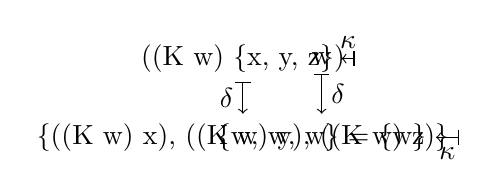
\begin{tikzpicture}
    \node (A) at (0,\h) {((K w) \{x, y, z\})};
    \node (B) at (\w,\h) {w}
      edge [<-|] node [above] {$\kappa$} (A);
    \node (C) at (0,0) {\{((K w) x), ((K w) y), ((K w) z)\}}
      edge [<-|] node [left] {$\delta$} (A);
    \node (D) at (\w,0) {\{w, w, w\} = \{w\}}
      edge [<-|] node [right] {$\delta$} (B)
      edge [<-|] node [below] {$\kappa$} (C);
  \end{tikzpicture}
  \def\w{8}\def\h{2}
  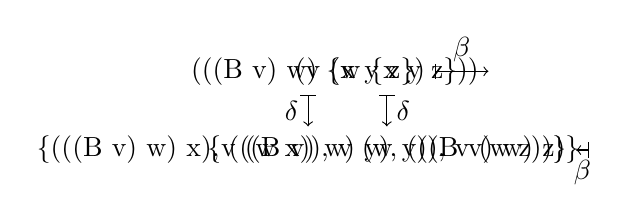
\begin{tikzpicture}
    \node (A) at (0,\h) {(((B v) w) \{x y z\})};
    \node (B) at (\w,\h) {(v (w \{x y z\}))}
      edge [<-|] node [above] {$\beta$} (A);
    \node (C) at (0,0) {\{(((B v) w) x), (((B v) w) y), (((B v) w) z)\}}
      edge [<-|] node [left] {$\delta$} (A);
    \node (D) at (\w,0) {\{v (w x)), v (w y)), v (w z))\}}
      edge [<-|] node [right] {$\delta$} (B)
      edge [<-|] node [below] {$\beta$} (C);
  \end{tikzpicture}
\caption{Using the ``sets of'' collection monad with the combinators $K$ and $B$.}
\label{fig:sets}
\end{figure*}




\begin{figure*}
\def\w{5}\def\h{2}
  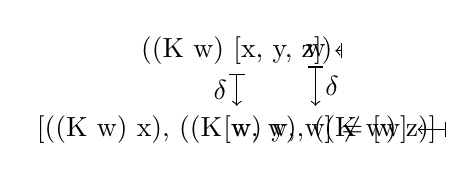
\begin{tikzpicture}
    \node (A) at (0,\h) {((K w) [x, y, z])};
    \node (B) at (\w,\h) {w}
      edge [<-|] (A);
    \node (C) at (0,0) {[((K w) x), ((K w) y), ((K w) z)]}
      edge [<-|] node [left] {$\delta$} (A);
    \node (D) at (\w,0) {[w, w, w] $\ne$ [w]}
      edge [<-|] node [right] {$\delta$} (B)
      edge [<-|] (C);
  \end{tikzpicture}

  \def\w{8}\def\h{2}
  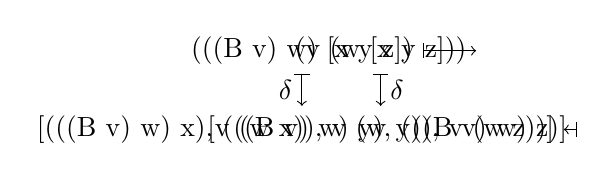
\begin{tikzpicture}
    \node (A) at (0,\h) {(((B v) w) [x y z])};
    \node (B) at (\w,\h) {(v (w [x y z]))}
      edge [<-|] (A);
    \node (C) at (0,0) {[(((B v) w) x), (((B v) w) y), (((B v) w) z)]}
      edge [<-|] node [left] {$\delta$} (A);
    \node (D) at (\w,0) {[v (w x)), v (w y)), v (w z))]}
      edge [<-|] node [right] {$\delta$} (B)
      edge [<-|] (C);
  \end{tikzpicture}
\caption{Using the ``lists of'' collection monad with the combinators $K$ and $B$.  Because $K$ discards information, there is no nontrivial distributive law for the $SKI$ calculus and the list monad.  The $BCI$ calculus, on the other hand, is linear, and works fine with the list monad.}
\label{fig:lists}
\end{figure*}

An operational semantics for a programming language needs to specify the grammar for the state of the computation, a structural equivalence, the reduction rules, and the reduction contexts.  There are various ways to model this in category theory.  One is by extending the multisorted Lawvere theory \cite{Trimble} of directed multigraphs with term constructors.  For example, we can model reduction of SKI terms to head normal form with the following presentation of a multisorted Lawvere theory:
\begin{enumerate}
  \item sorts $E, V$
  \item function symbols $s, t\maps E \to V$
  \item function symbols $S,K,I\maps 1 \to V$
  \item function symbols $S_1,K_1,I_1\maps 1 \to E$
  \item a function symbol $(-\;-)\maps V^2 \to V$
  \item a function symbol $(-\;-)_1\maps E\times V \to E$
  \item a function symbol $\sigma\maps V^3 \to V$
  \item a function symbol $\kappa\maps V^2 \to V$
  \item a function symbol $\iota\maps V\to V$
  \item an equation $s(\sigma(x,y,z)) = (((S\; x)\; y)\; z)$
  \item an equation $t(\sigma(x,y,z)) = ((x\; z)\;(y\; z))$
  \item an equation $s(\kappa(x,y,z)) = ((K\; x)\; z)$
  \item an equation $t(\kappa(x,y,z)) = x$
  \item an equation $s(\iota (x,y,z)) = (I\; z)$
  \item an equation $t(\iota (x,y,z)) = z$
\end{enumerate}
When we interpret this theory in Set, we get the set of edges and vertices in the graph of terms and rewrites, equipped with functions satisfying the equations.  Item 1 says that we have two generating objects in our theory, one for vertices and one for edges; the other objects of the theory include the terminal object 1 and those we get by taking products of objects.  Item 2 gives the source and target maps.  Item 3 says we have a chosen self edge on each vertex, a ``do nothing'' rewrite.  We include these so that the graph is the same as the one below.  Item 4 says that we have three generating vertices, one for each combinator.  Item 5 is a term constructor that lets us generate a new vertex by applying one vertex to another.  Item 6 says that the left side of an application is a reduction context.  Items 7-9 are the rewrites that generate the edges, and items 10-15 give the sources and targets of the rewrite rules.

Another way to model the SKI calculus is with a Gph-enriched Lawvere theory:
\begin{enumerate}
  \item a sort $G$
  \item function symbols $S,K,I\maps 1 \to G$
  \item a function symbol $(-\;-)\maps G^2 \to G$
  \item a function symbol $R\maps G \to G$
  \item an equation $R(x\; y) = (Rx\; y)$
  \item a rewrite $\sigma\maps R(((S\; x)\; y)\; z) \Rightarrow R((x\; z)\;(y\; z))$
  \item a rewrite $\kappa\maps R((K\; x)\; z) \Rightarrow Rx$
  \item a rewrite $\iota\maps R(I\; z) \Rightarrow Rz$
\end{enumerate}
Rather than interpret this theory in Set, we interpret it in Gph, the category of reflexive directed multigraphs.  We get a graph equipped with graph homomorphisms satisfying the equations and ``graph transformations'', the obvious analogy to natural transformations for graphs.  Item 1 says we have one generating object for the graph of terms and rewrites. Item 2 says we have one generating vertex with a chosen self edge for each combinator.  Item 3 says we can form new vertices by applying one vertex to another.  Item 4 is a reduction context marker.  We apply it to a term to mark the topmost context, since the fact that application is a graph homomorphism means that without a marker, if a rewrite can apply at some point in a term, it can apply at any point in the term.  Item 5 says that the left-hand side of an application is a reduction context.  Items 6-8 are the reduction rules and generate the edges of the graph.

The graph is the same in both cases, but each approach has its benefits.  The multisorted approach lets us write down formulae that use $s$ and $t$.  The Gph-enriched approach is much more concise, and lets us apply function symbols to entire graphs instead of just to edges.  Note that the category Gph, like Set, is a topos.

The kinds of theory mentioned above can only describe calculi without binders; for languages with binders, there are corresponding notions of nominal Lawvere theory \cite{GabbayPitts, Clouston}.

\section{Collections}

We follow Wadler \cite{Wadler} in thinking of collections as monads whose algebras have an annihilating element.  So far we have assumed that the collection monad acts on Set or Gph, but it's worth exploring the minimum requirements.  

Suppose that the one sort in the collection theory is $X.$  The annihilating element is picked out by a function symbol ${z\maps 1 \to X,}$ which means that the theory has to have a distinguished object 1, not necessarily terminal.  For the element to annihilate something, there must be some other function symbol ${m\maps X^{n \ge 2} \to X}$ for combining elements, which means that the theory has to have some notion of product, not necessarily cartesian.  Taken together, these mean the theory must be at least monoidal.  

If we don't care about the order of items in our collection, the theory should be symmetric monoidal.  If we want to be able to take a collection apart, then the theory needs projections, which forces the tensor product to be the categorical product and the distinguished object to be terminal.  We often want to model relations with collections; to do that, we need a transformation ${\rho\maps C(X\times Y) \to (X \to CY)}$ natural in $Y$ and dinatural in $X$ for mapping the ``collection of pairs'' view to the ``related elements'' view.  To support this, the theory must have internal homs.  

In what follows, we assume that the theory is cartesian closed and the collection supports all the features above.  The transformation $\rho$ means that there's a map from ${C(X)\cong C(X \times 1)}$ to ${X \to C1.}$  In the special case where $C$ is the covariant power monad, $C1$ is the subobject classifier $\Omega.$

\section{Formulae}

A mere Lawvere theory can be thought of as either a multisorted Lawvere theory with only one sort or as a Gph-enriched Lawvere theory with no edges.  In the former case, we sum the monads by identifying the one sort from the collection theory with the sort for edges and then taking the union of the sets of function symbols and the sets of equations.  In the latter case, there's no choice to make about which sorts to identify.

The logical operations on formulae are given by morphisms $C1^n \to C1$ for each $n.$  When $C$ is the monad for lists, for instance, $C1$ is isomorphic to the natural numbers, so we have a ``truth value'' for each natural number and operations like max and min, sum, absolute difference, and product.  Note that there is no ``completely true'' because infinity is not an element of the natural numbers.  Given any true statement (that is, not truth level 0), there are infinitely more that are ``more true.''

\section{Realization}

Given an object $X,$ a useful way to think of $(T+C)X$ is as
\[X + TX + CX + TTX + TCX + CTX + CCX + TTTX + \cdots.\]
That is, any interleaving of term calculus function symbols and collection symbols is allowed. Using the units and joins of $T$ and $C,$ we can coerce the term into the form $(TC)^nX$ for some $n.$  The distributive law then lets us move $T$s past $C$s so that all the $C$s are on the left of the $T$s, at which point we use the joins again to get a term in $CTX.$

A nontrivial distributive law does not always exist for a particular choice of $T$ and $C.$  In figures \ref{fig:sets} and \ref{fig:lists}, we show how the ``sets of'' collection monad admits both the linear BCI and nonlinear SKI combinators, but the ``lists of'' collection monad only admits linear ones.

\section{Typed terms}

Every term belongs to the singleton collection containing just itself, so every term is well-typed.  Every term context maps the term filling the hole to the term in contest, so every term context is a type constructor.  Using the example of the SKI calculus, the one-hole term context $(I\; -)$ is a type constructor taking any type $X$ to the type $(I\;X).$  

Note that the type $(I\;X)$ is not equivalent to the type $X$ in the theories described above.  It is an assertion about the actual shape of a term, up to structural equivalence; this makes sense to do because we are not modding out by rewrites.  In the case of confluent calculi like the SKI calculus, modding out by rewrites is harmless, but in the case of concurrent calculi like the pi calculus, it matters in what order reductions occur, so we can't mod out by them without destroying the intended semantics.

\section{Subtyping}

The elements of $C1$ form a partially ordered set; we say $c \le c'$ if $c$ is a subterm of $c'.$  As noted above, the elements do not necessarily form a lattice; when $C$ is the monad for lists, there is no longest list to contain all the others.  We do, however, always have an empty collection by assumption.

We can pull back the subtyping on collections of terms to formulae by means of the realization natural transformation, but sometimes that's unnecessary.  If we know that a type $X$ is a subtype of $Y,$ then for any one-hole formula context $K[-],$ the formula $K[X]$ is a subtype of $K[Y].$  The empty collection is, of course, a subtype of every other.

\section{Soundness and completeness}

Because we pull back the subtyping, the modality-free logic is sound by construction; because $CTX$ is a subset of $(T+C)X$ for all $X,$ the modality-free logic is complete.

\section{Modalities}

We can introduce the syntax for modalities with a third monad $M$ and define $T'$ as $T+M.$  We realize the modalities with a natural transformation $\Delta\maps M \to CT.$  The realization transformation for formulae with modalities factors as
\[ \begin{array}{rl}
  (T'+C) & \stackrel{\interp{-}}{\Rightarrow} CT' = C(T+M) \\
    & \stackrel{C(T+\Delta)}{\Rightarrow} CT+CCT = (C + CC)T \\
    & \stackrel{(C + \mu_C)T}{\Rightarrow} CT.
\end{array} \]
The first part of the transformation treats the modalities as atomic, leaving them unchanged; the second part interprets the modalities; and the third uses joins where necessary to get a single collection of terms.

The possibility modality $\diamond t$ can be realized as 
\[\{ t'\;|\; \exists t', \rho. s(\rho) = t' \land t(\rho) = t\}.\]  
The generalized possibility modality $X\langle K\rangle Y$ from the introduction can be realized as 
\[\{ t\;|\; \exists u:X, v:Y, \rho. s(\rho) = K[t, u] \land t(\rho) = v \}. \]
Note that these comprehensions only make sense when the notion of collection gives a lattice so that it makes sense to have the quantifier range over all the variables.  When that is not the case, we have to limit the scope to specific collections:
\[\diamond_{P,Q} t = \{ t'\;|\; \exists t':P, \rho:Q. s(\rho) = t' \land t(\rho) = t\}\]
\[\begin{array}{l}
  X\langle K,P,Q\rangle Y \\
  \quad = \{ t:P\;|\; \exists u:X, v:Y, \rho:Q. s(\rho) = K[t, u] \land t(\rho) = v \}.
\end{array} \]

As before, we can pull back the subtyping, so the resulting logic is sound; this time, however, it is not necessarily complete.

\section{Conclusion}

We presented an alternative approach to categorical logic based on monads and a distributive law.  The technique allows one to take a formal operational semantics of a programming language, a collection monad, and a distributive law and produce a structural-behavioral type system.  Such types have found application on the blockchain to prove the absence of race conditions in smart contracts \cite{PettersonMeredith}.

%% types are collections
%% unit type // must have empty collection
%% sorts are types (base collections)
%% product // must be free monoidal
%% internal hom // functions between collections
%% power objects // collections of collections
%% 
%% atomic formulae 
%% base relations A -> P1
%% equality AxA -> P1
%% inhabitation AxPA -> P1
%% 
%% terms
%% *:1, FV(*) = {}
%% const k:A, FV(k) = {}
%% var v:A, FV(v) = {v}
%% fn sym f:A -> B, term t:A => f(t):B, FV(f(t)) = FV(t)
%% s:A, t:B => <s,t>:AxB, FV(<s,t>) = FV(s) ∪ FV(t)
%% s:AxB => left(s):A, FV(left(s)) = FV(s)
%% s:AxB => right(s):B, FV(right(s)) = FV(s)
%% s:B, a:A => λa.s:[A -> B], FV(λa.s) = FV(s) - {a}
%% f:[A->B], t:A => ev(f,t):B, FV(ev(f,t):B) = FV(f) ∪ FV(t)
%% θ:P1, a:A => {a | θ}:P1, FV({a | θ}) = FV(θ) - {a} // special case of λ for B = P1

%% types
%% unit type I
%% sorts are types // sorts here are formulae
%% tensor product
%% internal hom
%% "power" monad P
%% 
%% atomic formulae
%% base relations A -> P1
%% equality A⊗A -> P1 // [] no otherwise yes
%% inhabitation A⊗PA -> P1 // [] no otherwise yes
%% 
%% terms
%% *:1, FV(*) = {}
%% const k:A, FV(k) = {}
%% var v:A, FV(v) = {v}
%% fn sym f:A -> B, term t:A => f(t):B, FV(f(t)) = FV(t)
%% s:A, t:B => <s,t>:A⊗B, FV(<s,t>) = FV(s) + FV(t)
%% s:ΓxA -> B, a:A => λa.s:[A -> B], FV(λa.s) = components(Γ)
%% f:[A->B], t:A => ev(f,t):B, FV(ev(f,t):B) = FV(f) + FV(t)
%% θ:ΓxA -> P1, a:A => {a | θ}:P1, FV({a | θ}) = components(Γ) // special case of λ for B = P1




%% ∃_f S = [ y∈Y | ∃x∈X. f(x)=y  ∧  x∈S ] = map f S
%% 
%% f:ℕ->[ℕ]
%% f(x) = [x] if x even, [] otherwise
%% How to write this?
%% x is ``even'' if there exists y st y+y = x
%% 
%% !:X -> 1
%% exists_! S = [•∈1 | ∃x∈X. !(x) = •  ∧  x in S] = S nonempty
%% 
%% S = [x'∈{x} | ∃y∈ℕ. y+y = x' ^ y∈ℕ ]
%% 
%% evens in S⊆ℕ: join [ y∈Y | ∃x:ℕ. f(x) = y  ∧  x ∈ S ] = [y | x <- S, y <- f(x)] = flatmap f S
%% 
%% inhabitation s in S = 1 if not, otherwise yes
%% 
%% ``set-like'' collections: P1 is a classifier 
%% 



%% Bibliography
%\bibliography{bibfile}
\begin{thebibliography}{99}
\bibitem{Clouston} Ranald Clouston, ``Nominal Lawvere Theories: A category theoretic account of equational theories with names'', {\em J. Comput. Syst. Sci.}, {\bf 80} (6), 1067--1086.

\bibitem{GabbayPitts} Murdoch Gabbay and Andrew M.~Pitts, ``A New Approach to Abstract Syntax with Variable Binding,'' {\em Formal Asp. Comput.} {\bf 13} (3-5), 341--363.

\bibitem{PettersonMeredith} Jack Petterson and Lucius Gregory Meredith, ``Notes on the DAO re-entrancy bug and behavioral types,'' \href{https://docs.google.com/document/d/1sGlObhGhoEizBXC30Ww4h1KHKGkmcy4NiCKitIBqiUg/edit}{https://docs.google.com/document/d/1sGlObhGhoEizBXC30Ww4h1KHKGkmcy4NiCKitIBqiUg/edit}.

\bibitem{Trimble} Todd Trimble, ``multisorted Lawvere theories,'' \href{https://ncatlab.org/toddtrimble/published/multisorted+Lawvere+theories}{https://ncatlab.org/toddtrimble/published/multisorted+Lawvere+theories}.

\bibitem{Wadler} Philip Wadler, ``Comprehending monads,'' {\em Proceedings of the 1990 ACM conference on LISP and functional programming (LFP),} 61--78.

\end{thebibliography}

%% Appendix
%%\appendix
%%\section{Appendix}

%% Text of appendix \ldots

\end{document}
